\documentclass[12pt]{article}
\usepackage[a4paper, margin=.30in]{geometry}
\usepackage{graphicx ,
            wrapfig,
            xcolor, 
            enumerate,
            amsmath,fontenc,
            tcolorbox,mathrsfs
            }
\usepackage{mathptmx}
\usepackage[siunitx, RPvoltages]{circuitikz}
\newcommand\headerMe[2]{\noindent{}#1\hfill#2}
\renewcommand{\thesection}{\Roman{section}}

\author{Zakaria HAOUZAN}
\date{\today}

\begin{document}
% headers --------------
\headerMe{Matière : Physique-Chimie}{Professeur : Zakaria HAOUZAN}\\
\headerMe{Unité : Electricité}{Établissement : Lycée SKHOR qualifiant}\\
\headerMe{Niveau : 1BAC-SM/X}{Heure : 17H/12H}\\

% ------Content ________

%\begin{wrapfigure}[10]{r}{0.5\textwidth}
    %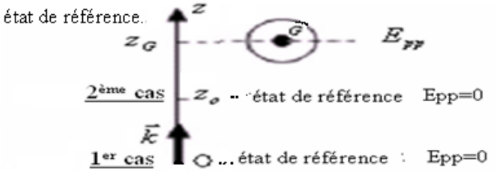
\includegraphics[width=0.5\textwidth]{./img/img00.png}
%\end{wrapfigure}


%\begin{tcolorbox}[colback=black!15!white,
                  %colframe=black!10!black,
                  %title=Remarque :
                 %]
\begin{center}

    \Large{Leçon $N^{\circ} 13 $: \color{red} Visibilité d'un Objet}
\end{center}

%\begin{wrapfigure}[5]{r}{0.3\textwidth}
  %\vspace{-3cm}
    %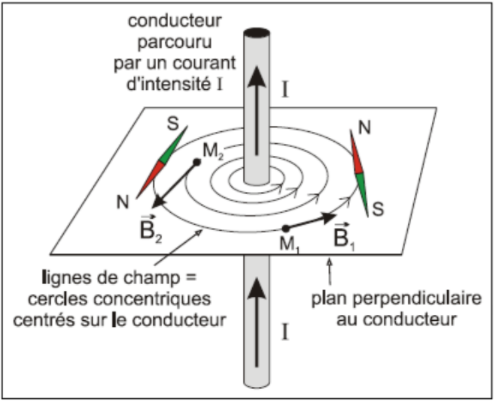
\includegraphics[width=0.3\textwidth]{./img/Un fil de longueur.png}
%\end{wrapfigure}
  \section{Conditions de visibilité d’un objet : }
1) Situation 1:

  Lorsqu'un observateur se trouve dans une pièce obscure,il ne voit rien.Pour pouvoir distinguer les objets présents autour
de lui Il doit allumer la lumière. Donc la visibilité d’un objet nécessite de la lumière.

2) Situation 2:

  Lorsqu'on place un objet et une bougie allumée dans une boite à chaussure de carton fermée ,on ne voit pas l'objet
malgré qu'il est éclairé.

  L'objet éclairé par une source de lumière primaire et lui aussi une source de lumière secondaire.

  La lumière émise par l'objet éclairé ne peut pas traverser les plaques de carton opaque pour arriver à l'œil de l'observateur.

3) Conclusion:

  Pour voir un objet,il doit être éclairé et l'œil de l'observateur doit recevoir la lumière diffusée par cet objet.

  \section{Propagation rectiligne de la lumière : modèle du rayon lumineux. }

  1)Expérience:

On dispose de trois plaques de carton percées d'un trou et d'une bougie alumée .
  \begin{center}
    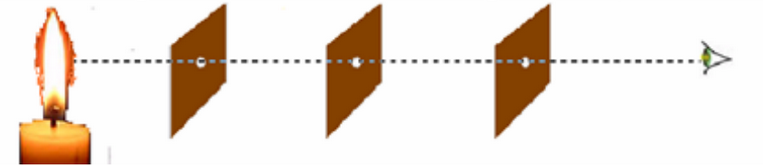
\includegraphics[width=0.3\textwidth]{./img/Optique_00.png}
\end{center}

Lorsque les trous sont alignés , l'œil observe la lumière de la bougie.

  2) Conclusion:

  Dans un milieu transparent et homogène la lumière se propage en ligne droite.
  \section{Réflexion de la lumière.}
  \subsection{Mise en évidence de la réflexion de la lumière:}
Lorsqu'on envoie un faisceau lumineux obliquement sur la surface réfléchissante d'un miroir plan horizontale , il se
réfléchit .
  \begin{center}
    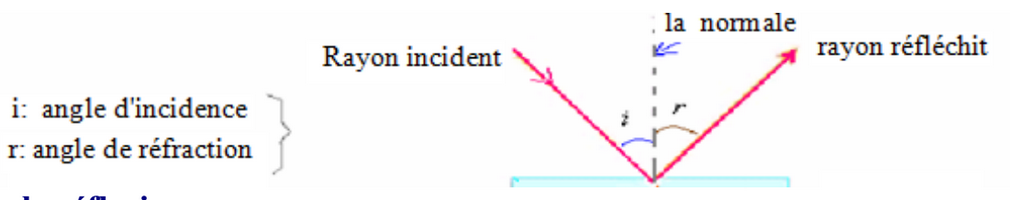
\includegraphics[width=0.6\textwidth]{./img/optique_01.png}
\end{center}

  \subsection{Lois de la réflexion: }
  \begin{tcolorbox}
  1ère loi : Le rayon incident , le rayon réfléchit et la normale au plan réfléchissant se trouvent dans le même plan.

    2ème loi: l'angle d'incidence est égale à l'angle de réflexion. (i=r).
  \end{tcolorbox}
  \begin{center}
    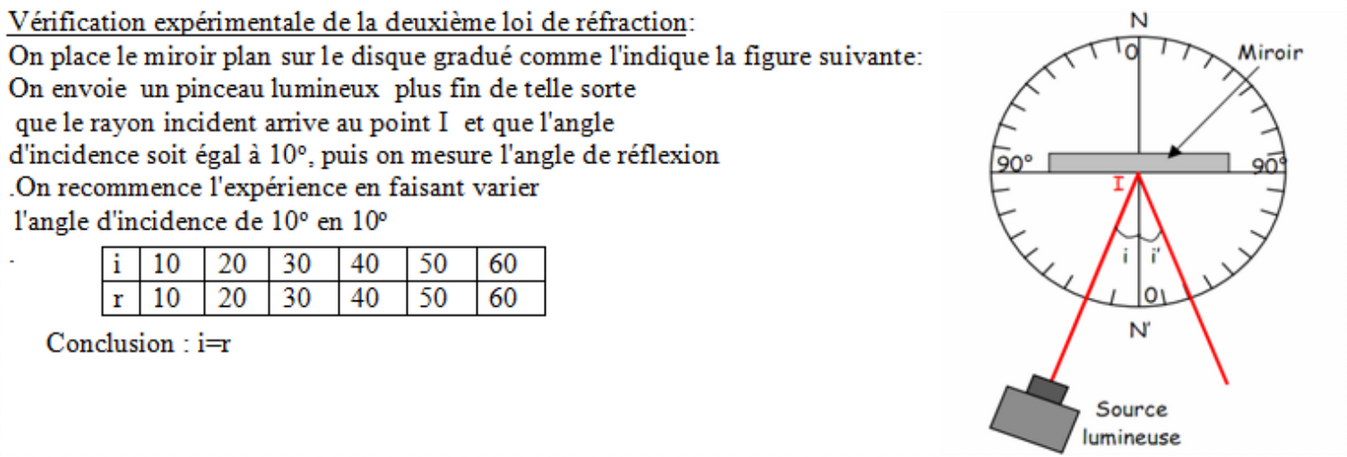
\includegraphics[width=1\textwidth]{./img/Optique_02.png}
\end{center}

  \section{Réfraction de la lumière.}
\subsection{Expérience du bâton brisé: }
On immerge partiellement un crayon dans un cristallisoir plein d'eau .
  \begin{center}
    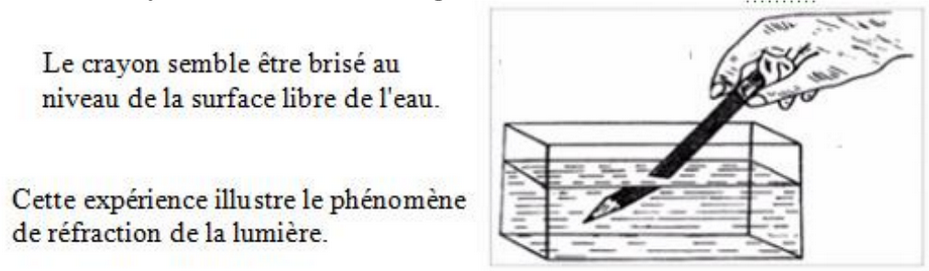
\includegraphics[width=0.5\textwidth]{./img/Optique_03.png}
\end{center}
\subsection{Définition: }
\begin{tcolorbox}
  On appelle réfraction de la lumière, le changement de direction qu'elle subit lorsqu'elle traverse la surface de séparation entre deux milieux transparents.
\end{tcolorbox}
\subsection{Vérification expérimentale de la 2ème loi la réfraction:}
  \begin{center}
    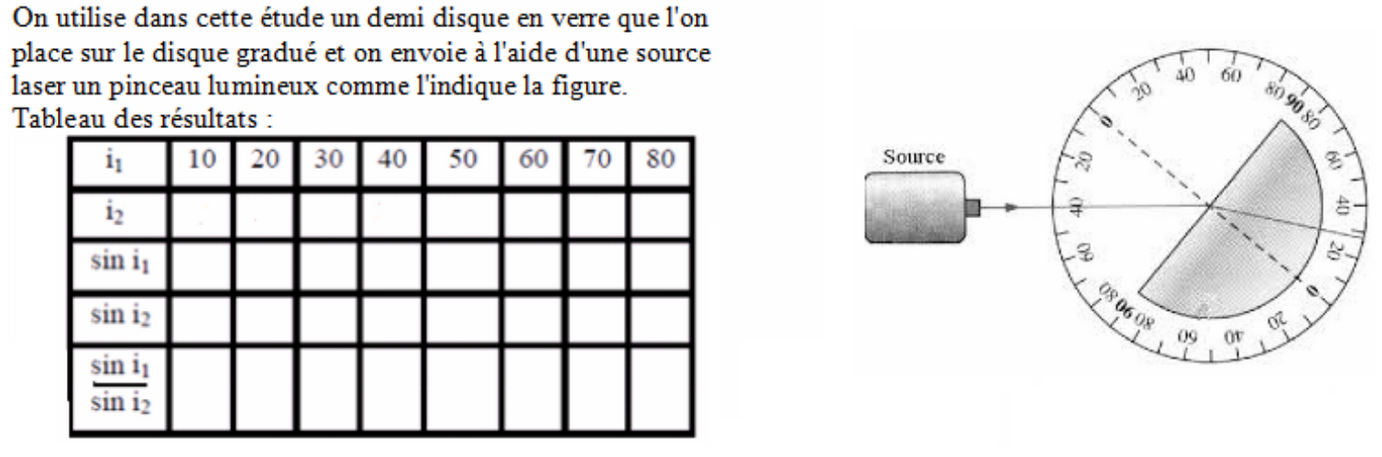
\includegraphics[width=0.9\textwidth]{./img/Optique_04.png}
\end{center}

On constate que le rapport :$\frac{sin(i_1)}{sin(i_2)}$
est constant, on le note $n_{2/1}$ c'est l'indice de réfraction du milieu 2 par rapport au milieu 1.

L'indice de réfraction absolu d'un milieu est son indice de réfraction relatif par rapport au vide , on le note n.

Exemple : l'indice de réfraction absolu de l'air est $n_{air}=1$ ,on l'appelle aussi indice de réfraction de l'air.

l'indice de réfraction absolu du verre est $n_{verre}=1,5$ , on l'appelle aussi indice de réfraction du verre.


( $n_1$: indice de réfraction du 1er milieu -  $n_2$ indice de réfraction du 2ème milieu). $n_{2/1} = \frac{n_2}{n_1}$

donc $n_1.sin(i_1) = n_2.sin(i_2)$


\end{document}

